\documentclass[11pt,letterpaper]{article}

%\usepackage[latin1]{inputenc} 
\usepackage[utf8]{inputenc}
\usepackage[cyr]{aeguill}
\usepackage[colorlinks=true]{hyperref}
\usepackage{textpos}
\usepackage{graphicx}
\usepackage[french]{babel}
\usepackage{color}
\usepackage{array}
\usepackage{enumerate}
\usepackage{fancyhdr}
\usepackage{lastpage}
\usepackage{amsmath}
\usepackage{amssymb}
\usepackage{epstopdf}
\usepackage{mathrsfs}
\usepackage{float}
\usepackage{caption}
\usepackage{subcaption}
\usepackage{siunitx}
\addto\captionsfrench{\def\tablename{Tableau}}

%-----------------------------------------------------------------%
% Definitions
\newcommand{\session}{Hiver 2022}
\newcommand{\firstauthor}{Yoan \textbf{Fournier}}
\newcommand{\firstregistrationnumber}{1958736}
\newcommand{\secondauthor}{Victor \textbf{Gaudreau-Blouin}}
\newcommand{\secondregistrationnumber}{??????}
\newcommand{\reportnumber}{}
\newcommand{\firsttitle}{???Analyse énergétique d'un processeur vectoriel pour des calculs de DNN???}
\newcommand{\secondtitle}{Proposition}
%-----------------------------------------------------------------%



\oddsidemargin 0pt
\topmargin 0pt
\textwidth 6.5in
\textheight 8.1in

\setlength{\parskip}{1em}

\definecolor{bleu_poly}{RGB}{65,170,230}
\definecolor{vert_poly}{RGB}{140,200,60}
\definecolor{orange_poly}{RGB}{250,150,30}
\definecolor{rouge_poly}{RGB}{185,30,50}
\definecolor{gris_poly}{RGB}{166,168,171}


\title{\vspace{-2.5cm} \noindent\makebox[\linewidth]{\color{rouge_poly}{\rule{\textwidth}{1.5pt}}}
        \begin{center}
        \begin{tabular}{m{6.5cm}m{6cm}}
        \textbf{ \huge Projet \reportnumber}  & 
\includegraphics[width=0.4\textwidth]{Polytechnique_signature-CMYK-droite_FR.eps}
        \end{tabular}
        \end{center}
        \noindent\makebox[\linewidth]{\color{rouge_poly}{\rule{\textwidth}{1.5pt}}}
        \\ \  \\
        \Huge \firsttitle \\ \secondtitle  
        \\ \ \\
        \LARGE ELE6307 - Machines neuronales : architectures et applications
        }

\author{\session \\ Département de génie électrique \\ École Polytechnique de Montréal} 

\date{Dernière mise à jour: \today}

\pagestyle{fancy}

\lfoot{\session}
\cfoot{ELE6307 - Machines neuronales : architectures et applications}
\rfoot{\thepage/\pageref{LastPage}}
\chead{}
\lhead{\emph{Projet -- \firstauthor  \, (\firstregistrationnumber)/\secondauthor\,  (\secondregistrationnumber)}}
\rhead{
\includegraphics[width=2.5cm]{Polytechnique_signature-CMYK-droite_FR.eps}}
\renewcommand{\headrulewidth}{0.4pt}
\renewcommand{\footrulewidth}{0.4pt} 
\setlength{\headheight}{45pt}


\graphicspath{{fig/}}


\newcommand{\vb}[1]{\mathbf{#1}}
\newcommand{\bs}[1]{\boldsymbol{#1}}


%-----------------------------------------------------------------%
% SOF
\begin{document}
\maketitle
\noindent\makebox[\linewidth]{\color{rouge_poly}{\rule{\textwidth}{1.5pt}}} 


\noindent \LARGE \firstauthor  \hfill \firstregistrationnumber


\noindent \LARGE \secondauthor \hfill \secondregistrationnumber


\noindent\makebox[\linewidth]{\color{rouge_poly}{\rule{\textwidth}{1.5pt}}}


\newpage
\normalsize

\section*{Présentation du sujet}
    Dans les dernières années, l'utilisation de réseaux de neurones profonds (DNN) pour
    résoudre différentes tâches a beaucoup augmenté. Ces DNNs nécessitent des puissances
    de calculs considérables, mais à la fois nécessitent une bonne efficacité énergétique 
    étant donné leur déploiement dans des appareils mobiles. Bien que les processeurs 
    généralistes que l'on retrouve aujourd'hui ont augmenté rapidement en performance,
    les limitations du \textit{Dennard Scaling} se font ressentir. Il est donc souhaitable
    de trouver une autre approche pour accélérer de façon efficace les calculs dans les DNNs.
    Une manière intéressante pour l'accélération des calculs pour des DNNs est l'utilisation
    de processeurs vectoriels plutôt que des processeurs scalaires standards. Ces processeurs
    utilisent un jeu d'instruction SIMD (\textit{Single instruction, Multiple Data}) plutôt 
    que SISD (\textit{Single instruction, Single data}). Ainsi une instruction SIMD peut
    performer la même opération sur plusieurs données plutôt qu'une seule, ce qui permet 
    de plus facilement augmenter le parallélisme des calculs. Le projet proposé vise donc 
    à étudier l'efficacité énergétique pour différentes configurations de processeurs 
    vectoriels en comparant cette efficacité avec une architecture de processeur scalaire 
    standard.

\section*{Méthodologie}
    L'architecture sur laquelle se basera notre modélisation est sur celle du coprocesseur 
    vectoriel ARA \cite{ara_paper}. Ce coprocesseur est une extension vectorielle du processeur scalaire
    RISCV CVA6. Le fonctionnement d’ARA se base sur le concept de \textit{Lanes}. 
    La figure \ref{fig:ara_arch} présente l'architecture d’ARA \cite{bougenot_2020}. %TODO: Explication de l'arch

    La première étape du projet visera à modéliser l'architecture d'une \textit{Lane} à
    l'aide de Timeloop/Accelergy \cite{timeloop}. %TODO: présenté timeloop accerlegy real quick
    L'architecture présentée à la figure \ref{fig:lane_arch}
    est plutôt complexe, mais elle peut, à sa plus simple expression, être modélisée comme
    un PE avec une mémoire locale de 8 données. Ainsi, par la suite, l'architecture globale
    sera modélisée en combinant un nombre paramétrable de \textit{Lanes} à une mémoire globale.
    Le processeur scalaire, lui peut être modélisé en utilisant une seule \textit{Lane}.

    La deuxième étape utilisera \textit{timeloop mapper} afin de venir analyser la consommation
    énergétique de l'architecture pour un problème standard de convolution comme, par exemple,
    une des couches convolutives du DNN VGG16. La consommation sera évaluée pour 2, 4, 8 et 16 
    \textit{Lanes}. Ensuite, d'autres paramètres comme la taille en bits des poids pourront
    être modifiés afin d'évaluer leur impact sur la performance énergétique.

    % TODO: Calcul GFLOP/W
    

\section*{Objectifs et résultats}
    L'objectif du projet et de comparer l'efficacité et l'évolutivité d'un processeur 
    vectoriel vis-à-vis un processeur scalaire plus standard pour les types de calculs
    principalement utilisés dans des DNNs. Le projet vise à démontrer qu'il est avantageux
    d'opter pour une architecture vectorielle.

    Les résultats présentés seront les mesures d'efficacité énergétique en GFLOP/W pour
    un processeur scalaire (1 \text{Lanes}) et un processeur vectoriel à (2, 4, 8, 16 \text{Lanes}).

{\bibliography{refs}}
    \bibliographystyle{abbrv}

\section*{Annexes}
    \begin{figure}[H]
        \begin{subfigure}{.5\textwidth}
        \centering
        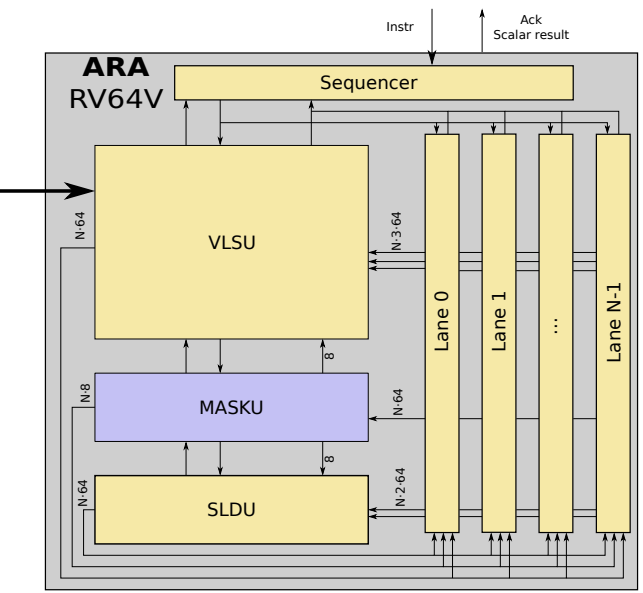
\includegraphics[width=1.1\linewidth]{ara_arch.png}
        \caption{Arch. globale}
        \label{fig:top_arch}
        \end{subfigure}%
        \begin{subfigure}{.5\textwidth}
        \centering
        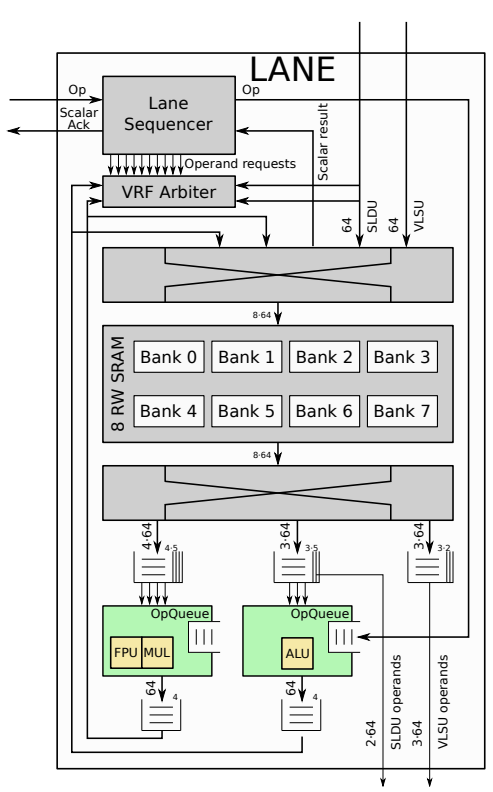
\includegraphics[width=.65\linewidth]{lane_arch.png}
        \caption{Arch. \textit{Lane}}
        \label{fig:lane_arch}
        \end{subfigure}
        \caption{Architecture d'ARA}
        \label{fig:ara_arch}
    \end{figure}

\end{document} 
%-----------------------------------------------------------------%
% EOF